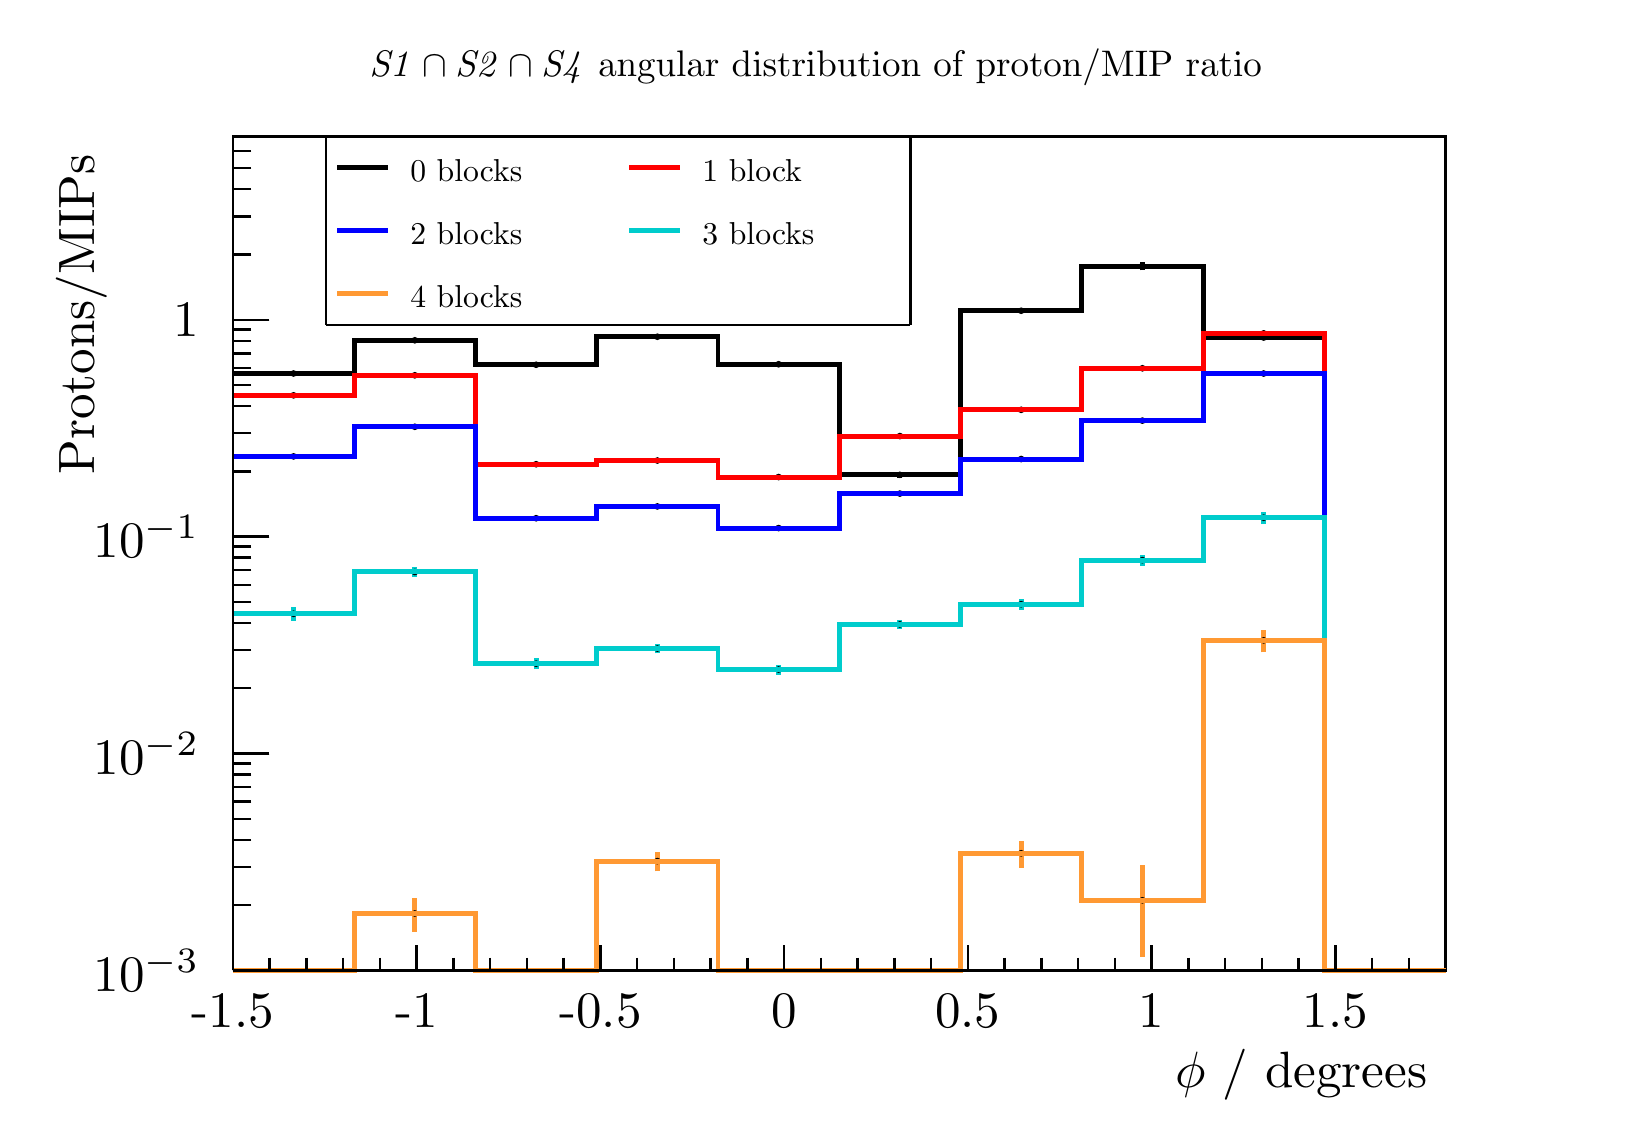
\begin{tikzpicture}
\pgfdeclareplotmark{cross} {
\pgfpathmoveto{\pgfpoint{-0.3\pgfplotmarksize}{\pgfplotmarksize}}
\pgfpathlineto{\pgfpoint{+0.3\pgfplotmarksize}{\pgfplotmarksize}}
\pgfpathlineto{\pgfpoint{+0.3\pgfplotmarksize}{0.3\pgfplotmarksize}}
\pgfpathlineto{\pgfpoint{+1\pgfplotmarksize}{0.3\pgfplotmarksize}}
\pgfpathlineto{\pgfpoint{+1\pgfplotmarksize}{-0.3\pgfplotmarksize}}
\pgfpathlineto{\pgfpoint{+0.3\pgfplotmarksize}{-0.3\pgfplotmarksize}}
\pgfpathlineto{\pgfpoint{+0.3\pgfplotmarksize}{-1.\pgfplotmarksize}}
\pgfpathlineto{\pgfpoint{-0.3\pgfplotmarksize}{-1.\pgfplotmarksize}}
\pgfpathlineto{\pgfpoint{-0.3\pgfplotmarksize}{-0.3\pgfplotmarksize}}
\pgfpathlineto{\pgfpoint{-1.\pgfplotmarksize}{-0.3\pgfplotmarksize}}
\pgfpathlineto{\pgfpoint{-1.\pgfplotmarksize}{0.3\pgfplotmarksize}}
\pgfpathlineto{\pgfpoint{-0.3\pgfplotmarksize}{0.3\pgfplotmarksize}}
\pgfpathclose
\pgfusepathqstroke
}
\pgfdeclareplotmark{cross*} {
\pgfpathmoveto{\pgfpoint{-0.3\pgfplotmarksize}{\pgfplotmarksize}}
\pgfpathlineto{\pgfpoint{+0.3\pgfplotmarksize}{\pgfplotmarksize}}
\pgfpathlineto{\pgfpoint{+0.3\pgfplotmarksize}{0.3\pgfplotmarksize}}
\pgfpathlineto{\pgfpoint{+1\pgfplotmarksize}{0.3\pgfplotmarksize}}
\pgfpathlineto{\pgfpoint{+1\pgfplotmarksize}{-0.3\pgfplotmarksize}}
\pgfpathlineto{\pgfpoint{+0.3\pgfplotmarksize}{-0.3\pgfplotmarksize}}
\pgfpathlineto{\pgfpoint{+0.3\pgfplotmarksize}{-1.\pgfplotmarksize}}
\pgfpathlineto{\pgfpoint{-0.3\pgfplotmarksize}{-1.\pgfplotmarksize}}
\pgfpathlineto{\pgfpoint{-0.3\pgfplotmarksize}{-0.3\pgfplotmarksize}}
\pgfpathlineto{\pgfpoint{-1.\pgfplotmarksize}{-0.3\pgfplotmarksize}}
\pgfpathlineto{\pgfpoint{-1.\pgfplotmarksize}{0.3\pgfplotmarksize}}
\pgfpathlineto{\pgfpoint{-0.3\pgfplotmarksize}{0.3\pgfplotmarksize}}
\pgfpathclose
\pgfusepathqfillstroke
}
\pgfdeclareplotmark{newstar} {
\pgfpathmoveto{\pgfqpoint{0pt}{\pgfplotmarksize}}
\pgfpathlineto{\pgfqpointpolar{44}{0.5\pgfplotmarksize}}
\pgfpathlineto{\pgfqpointpolar{18}{\pgfplotmarksize}}
\pgfpathlineto{\pgfqpointpolar{-20}{0.5\pgfplotmarksize}}
\pgfpathlineto{\pgfqpointpolar{-54}{\pgfplotmarksize}}
\pgfpathlineto{\pgfqpointpolar{-90}{0.5\pgfplotmarksize}}
\pgfpathlineto{\pgfqpointpolar{234}{\pgfplotmarksize}}
\pgfpathlineto{\pgfqpointpolar{198}{0.5\pgfplotmarksize}}
\pgfpathlineto{\pgfqpointpolar{162}{\pgfplotmarksize}}
\pgfpathlineto{\pgfqpointpolar{134}{0.5\pgfplotmarksize}}
\pgfpathclose
\pgfusepathqstroke
}
\pgfdeclareplotmark{newstar*} {
\pgfpathmoveto{\pgfqpoint{0pt}{\pgfplotmarksize}}
\pgfpathlineto{\pgfqpointpolar{44}{0.5\pgfplotmarksize}}
\pgfpathlineto{\pgfqpointpolar{18}{\pgfplotmarksize}}
\pgfpathlineto{\pgfqpointpolar{-20}{0.5\pgfplotmarksize}}
\pgfpathlineto{\pgfqpointpolar{-54}{\pgfplotmarksize}}
\pgfpathlineto{\pgfqpointpolar{-90}{0.5\pgfplotmarksize}}
\pgfpathlineto{\pgfqpointpolar{234}{\pgfplotmarksize}}
\pgfpathlineto{\pgfqpointpolar{198}{0.5\pgfplotmarksize}}
\pgfpathlineto{\pgfqpointpolar{162}{\pgfplotmarksize}}
\pgfpathlineto{\pgfqpointpolar{134}{0.5\pgfplotmarksize}}
\pgfpathclose
\pgfusepathqfillstroke
}
\definecolor{c}{rgb}{1,1,1};
\draw [color=c, fill=c] (0,0) rectangle (20,13.7536);
\draw [color=c, fill=c] (2.6,1.78797) rectangle (18,12.3782);
\definecolor{c}{rgb}{0,0,0};
\draw [c,line width=0.9] (2.6,1.78797) -- (2.6,12.3782) -- (18,12.3782) -- (18,1.78797) -- (2.6,1.78797);
\definecolor{c}{rgb}{1,1,1};
\draw [color=c, fill=c] (2.6,1.78797) rectangle (18,12.3782);
\definecolor{c}{rgb}{0,0,0};
\draw [c,line width=0.9] (2.6,1.78797) -- (2.6,12.3782) -- (18,12.3782) -- (18,1.78797) -- (2.6,1.78797);
\definecolor{c}{rgb}{0,0,0.6};
\draw [c,line width=0.9] (2.6,1.78797) -- (4.14,1.78797) -- (4.14,1.78797) -- (5.68,1.78797) -- (5.68,1.78797) -- (7.22,1.78797) -- (7.22,1.78797) -- (8.76,1.78797) -- (8.76,1.78797) -- (10.3,1.78797) -- (10.3,1.78797) -- (11.84,1.78797) --
 (11.84,1.78797) -- (13.38,1.78797) -- (13.38,1.78797) -- (14.92,1.78797) -- (14.92,1.78797) -- (16.46,1.78797) -- (16.46,1.78797) -- (18,1.78797);
\definecolor{c}{rgb}{0,0,0};
\draw [c,line width=0.9] (2.6,1.78797) -- (18,1.78797);
\draw [c,line width=0.9] (2.6,2.10567) -- (2.6,1.78797);
\draw [c,line width=0.9] (3.06667,1.94682) -- (3.06667,1.78797);
\draw [c,line width=0.9] (3.53333,1.94682) -- (3.53333,1.78797);
\draw [c,line width=0.9] (4,1.94682) -- (4,1.78797);
\draw [c,line width=0.9] (4.46667,1.94682) -- (4.46667,1.78797);
\draw [c,line width=0.9] (4.93333,2.10567) -- (4.93333,1.78797);
\draw [c,line width=0.9] (5.4,1.94682) -- (5.4,1.78797);
\draw [c,line width=0.9] (5.86667,1.94682) -- (5.86667,1.78797);
\draw [c,line width=0.9] (6.33333,1.94682) -- (6.33333,1.78797);
\draw [c,line width=0.9] (6.8,1.94682) -- (6.8,1.78797);
\draw [c,line width=0.9] (7.26667,2.10567) -- (7.26667,1.78797);
\draw [c,line width=0.9] (7.73333,1.94682) -- (7.73333,1.78797);
\draw [c,line width=0.9] (8.2,1.94682) -- (8.2,1.78797);
\draw [c,line width=0.9] (8.66667,1.94682) -- (8.66667,1.78797);
\draw [c,line width=0.9] (9.13333,1.94682) -- (9.13333,1.78797);
\draw [c,line width=0.9] (9.6,2.10567) -- (9.6,1.78797);
\draw [c,line width=0.9] (10.0667,1.94682) -- (10.0667,1.78797);
\draw [c,line width=0.9] (10.5333,1.94682) -- (10.5333,1.78797);
\draw [c,line width=0.9] (11,1.94682) -- (11,1.78797);
\draw [c,line width=0.9] (11.4667,1.94682) -- (11.4667,1.78797);
\draw [c,line width=0.9] (11.9333,2.10567) -- (11.9333,1.78797);
\draw [c,line width=0.9] (12.4,1.94682) -- (12.4,1.78797);
\draw [c,line width=0.9] (12.8667,1.94682) -- (12.8667,1.78797);
\draw [c,line width=0.9] (13.3333,1.94682) -- (13.3333,1.78797);
\draw [c,line width=0.9] (13.8,1.94682) -- (13.8,1.78797);
\draw [c,line width=0.9] (14.2667,2.10567) -- (14.2667,1.78797);
\draw [c,line width=0.9] (14.7333,1.94682) -- (14.7333,1.78797);
\draw [c,line width=0.9] (15.2,1.94682) -- (15.2,1.78797);
\draw [c,line width=0.9] (15.6667,1.94682) -- (15.6667,1.78797);
\draw [c,line width=0.9] (16.1333,1.94682) -- (16.1333,1.78797);
\draw [c,line width=0.9] (16.6,2.10567) -- (16.6,1.78797);
\draw [c,line width=0.9] (16.6,2.10567) -- (16.6,1.78797);
\draw [c,line width=0.9] (17.0667,1.94682) -- (17.0667,1.78797);
\draw [c,line width=0.9] (17.5333,1.94682) -- (17.5333,1.78797);
\draw [anchor=base] (2.6,1.05903) node[scale=1.84551, color=c, rotate=0]{-1.5};
\draw [anchor=base] (4.93333,1.05903) node[scale=1.84551, color=c, rotate=0]{-1};
\draw [anchor=base] (7.26667,1.05903) node[scale=1.84551, color=c, rotate=0]{-0.5};
\draw [anchor=base] (9.6,1.05903) node[scale=1.84551, color=c, rotate=0]{0};
\draw [anchor=base] (11.9333,1.05903) node[scale=1.84551, color=c, rotate=0]{0.5};
\draw [anchor=base] (14.2667,1.05903) node[scale=1.84551, color=c, rotate=0]{1};
\draw [anchor=base] (16.6,1.05903) node[scale=1.84551, color=c, rotate=0]{1.5};
\draw [anchor= east] (18,0.467622) node[scale=1.84551, color=c, rotate=0]{$\phi$ / degrees};
\draw [c,line width=0.9] (2.6,1.78797) -- (2.6,12.3782);
\draw [c,line width=0.9] (3.062,1.78797) -- (2.6,1.78797);
\draw [anchor= east] (2.404,1.78797) node[scale=1.84551, color=c, rotate=0]{$10^{-3}$};
\draw [c,line width=0.9] (2.831,2.61707) -- (2.6,2.61707);
\draw [c,line width=0.9] (2.831,3.10207) -- (2.6,3.10207);
\draw [c,line width=0.9] (2.831,3.44618) -- (2.6,3.44618);
\draw [c,line width=0.9] (2.831,3.71309) -- (2.6,3.71309);
\draw [c,line width=0.9] (2.831,3.93117) -- (2.6,3.93117);
\draw [c,line width=0.9] (2.831,4.11556) -- (2.6,4.11556);
\draw [c,line width=0.9] (2.831,4.27528) -- (2.6,4.27528);
\draw [c,line width=0.9] (2.831,4.41616) -- (2.6,4.41616);
\draw [c,line width=0.9] (3.062,4.54219) -- (2.6,4.54219);
\draw [anchor= east] (2.404,4.54219) node[scale=1.84551, color=c, rotate=0]{$10^{-2}$};
\draw [c,line width=0.9] (2.831,5.37129) -- (2.6,5.37129);
\draw [c,line width=0.9] (2.831,5.85629) -- (2.6,5.85629);
\draw [c,line width=0.9] (2.831,6.2004) -- (2.6,6.2004);
\draw [c,line width=0.9] (2.831,6.46731) -- (2.6,6.46731);
\draw [c,line width=0.9] (2.831,6.68539) -- (2.6,6.68539);
\draw [c,line width=0.9] (2.831,6.86978) -- (2.6,6.86978);
\draw [c,line width=0.9] (2.831,7.0295) -- (2.6,7.0295);
\draw [c,line width=0.9] (2.831,7.17039) -- (2.6,7.17039);
\draw [c,line width=0.9] (3.062,7.29641) -- (2.6,7.29641);
\draw [anchor= east] (2.404,7.29641) node[scale=1.84551, color=c, rotate=0]{$10^{-1}$};
\draw [c,line width=0.9] (2.831,8.12552) -- (2.6,8.12552);
\draw [c,line width=0.9] (2.831,8.61051) -- (2.6,8.61051);
\draw [c,line width=0.9] (2.831,8.95462) -- (2.6,8.95462);
\draw [c,line width=0.9] (2.831,9.22153) -- (2.6,9.22153);
\draw [c,line width=0.9] (2.831,9.43962) -- (2.6,9.43962);
\draw [c,line width=0.9] (2.831,9.624) -- (2.6,9.624);
\draw [c,line width=0.9] (2.831,9.78372) -- (2.6,9.78372);
\draw [c,line width=0.9] (2.831,9.92461) -- (2.6,9.92461);
\draw [c,line width=0.9] (3.062,10.0506) -- (2.6,10.0506);
\draw [anchor= east] (2.404,10.0506) node[scale=1.84551, color=c, rotate=0]{1};
\draw [c,line width=0.9] (2.831,10.8797) -- (2.6,10.8797);
\draw [c,line width=0.9] (2.831,11.3647) -- (2.6,11.3647);
\draw [c,line width=0.9] (2.831,11.7088) -- (2.6,11.7088);
\draw [c,line width=0.9] (2.831,11.9758) -- (2.6,11.9758);
\draw [c,line width=0.9] (2.831,12.1938) -- (2.6,12.1938);
\draw [c,line width=0.9] (2.831,12.3782) -- (2.6,12.3782);
\draw [anchor= east] (0.68,12.3782) node[scale=1.84551, color=c, rotate=90]{ Protons/MIPs};
\draw [c,line width=1.8] (3.37,9.33443) -- (3.37,9.36864);
\draw [c,line width=1.8] (3.37,9.36864) -- (3.37,9.40191);
\foreach \P in {(3.37,9.36864)}{\draw[mark options={color=c,fill=c},mark size=2.402402pt,mark=*,mark size=1pt] plot coordinates {\P};}
\draw [c,line width=1.8] (4.91,9.77172) -- (4.91,9.79023);
\draw [c,line width=1.8] (4.91,9.79023) -- (4.91,9.80845);
\foreach \P in {(4.91,9.79023)}{\draw[mark options={color=c,fill=c},mark size=2.402402pt,mark=*,mark size=1pt] plot coordinates {\P};}
\draw [c,line width=1.8] (6.45,9.45426) -- (6.45,9.47943);
\draw [c,line width=1.8] (6.45,9.47943) -- (6.45,9.50408);
\foreach \P in {(6.45,9.47943)}{\draw[mark options={color=c,fill=c},mark size=2.402402pt,mark=*,mark size=1pt] plot coordinates {\P};}
\draw [c,line width=1.8] (7.99,9.8212) -- (7.99,9.83547);
\draw [c,line width=1.8] (7.99,9.83547) -- (7.99,9.84956);
\foreach \P in {(7.99,9.83547)}{\draw[mark options={color=c,fill=c},mark size=2.402402pt,mark=*,mark size=1pt] plot coordinates {\P};}
\draw [c,line width=1.8] (9.53,9.46297) -- (9.53,9.48602);
\draw [c,line width=1.8] (9.53,9.48602) -- (9.53,9.50864);
\foreach \P in {(9.53,9.48602)}{\draw[mark options={color=c,fill=c},mark size=2.402402pt,mark=*,mark size=1pt] plot coordinates {\P};}
\draw [c,line width=1.8] (11.07,8.04764) -- (11.07,8.08165);
\draw [c,line width=1.8] (11.07,8.08165) -- (11.07,8.11473);
\foreach \P in {(11.07,8.08165)}{\draw[mark options={color=c,fill=c},mark size=2.402402pt,mark=*,mark size=1pt] plot coordinates {\P};}
\draw [c,line width=1.8] (12.61,10.1518) -- (12.61,10.1655);
\draw [c,line width=1.8] (12.61,10.1655) -- (12.61,10.179);
\foreach \P in {(12.61,10.1655)}{\draw[mark options={color=c,fill=c},mark size=2.402402pt,mark=*,mark size=1pt] plot coordinates {\P};}
\draw [c,line width=1.8] (14.15,10.6794) -- (14.15,10.7336);
\draw [c,line width=1.8] (14.15,10.7336) -- (14.15,10.7854);
\foreach \P in {(14.15,10.7336)}{\draw[mark options={color=c,fill=c},mark size=2.402402pt,mark=*,mark size=1pt] plot coordinates {\P};}
\draw [c,line width=1.8] (15.69,9.79912) -- (15.69,9.82513);
\draw [c,line width=1.8] (15.69,9.82513) -- (15.69,9.85059);
\foreach \P in {(15.69,9.82513)}{\draw[mark options={color=c,fill=c},mark size=2.402402pt,mark=*,mark size=1pt] plot coordinates {\P};}
\draw [c,line width=1.8] (2.6,9.36864) -- (4.14,9.36864) -- (4.14,9.79023) -- (5.68,9.79023) -- (5.68,9.47943) -- (7.22,9.47943) -- (7.22,9.83547) -- (8.76,9.83547) -- (8.76,9.48602) -- (10.3,9.48602) -- (10.3,8.08165) -- (11.84,8.08165) --
 (11.84,10.1655) -- (13.38,10.1655) -- (13.38,10.7336) -- (14.92,10.7336) -- (14.92,9.82513) -- (16.46,9.82513) -- (16.46,1.78797) -- (18,1.78797);
\definecolor{c}{rgb}{1,0,0};
\draw [c,line width=1.8] (3.37,9.06638) -- (3.37,9.09098);
\draw [c,line width=1.8] (3.37,9.09098) -- (3.37,9.11508);
\definecolor{c}{rgb}{0,0,0};
\foreach \P in {(3.37,9.09098)}{\draw[mark options={color=c,fill=c},mark size=2.402402pt,mark=*,mark size=1pt] plot coordinates {\P};}
\definecolor{c}{rgb}{1,0,0};
\draw [c,line width=1.8] (4.91,9.32697) -- (4.91,9.3457);
\draw [c,line width=1.8] (4.91,9.3457) -- (4.91,9.36414);
\definecolor{c}{rgb}{0,0,0};
\foreach \P in {(4.91,9.3457)}{\draw[mark options={color=c,fill=c},mark size=2.402402pt,mark=*,mark size=1pt] plot coordinates {\P};}
\definecolor{c}{rgb}{1,0,0};
\draw [c,line width=1.8] (6.45,8.19237) -- (6.45,8.21622);
\draw [c,line width=1.8] (6.45,8.21622) -- (6.45,8.23961);
\definecolor{c}{rgb}{0,0,0};
\foreach \P in {(6.45,8.21622)}{\draw[mark options={color=c,fill=c},mark size=2.402402pt,mark=*,mark size=1pt] plot coordinates {\P};}
\definecolor{c}{rgb}{1,0,0};
\draw [c,line width=1.8] (7.99,8.24184) -- (7.99,8.26356);
\draw [c,line width=1.8] (7.99,8.26356) -- (7.99,8.2849);
\definecolor{c}{rgb}{0,0,0};
\foreach \P in {(7.99,8.26356)}{\draw[mark options={color=c,fill=c},mark size=2.402402pt,mark=*,mark size=1pt] plot coordinates {\P};}
\definecolor{c}{rgb}{1,0,0};
\draw [c,line width=1.8] (9.53,8.0303) -- (9.53,8.05327);
\draw [c,line width=1.8] (9.53,8.05327) -- (9.53,8.0758);
\definecolor{c}{rgb}{0,0,0};
\foreach \P in {(9.53,8.05327)}{\draw[mark options={color=c,fill=c},mark size=2.402402pt,mark=*,mark size=1pt] plot coordinates {\P};}
\definecolor{c}{rgb}{1,0,0};
\draw [c,line width=1.8] (11.07,8.55281) -- (11.07,8.57361);
\draw [c,line width=1.8] (11.07,8.57361) -- (11.07,8.59404);
\definecolor{c}{rgb}{0,0,0};
\foreach \P in {(11.07,8.57361)}{\draw[mark options={color=c,fill=c},mark size=2.402402pt,mark=*,mark size=1pt] plot coordinates {\P};}
\definecolor{c}{rgb}{1,0,0};
\draw [c,line width=1.8] (12.61,8.88516) -- (12.61,8.90743);
\draw [c,line width=1.8] (12.61,8.90743) -- (12.61,8.9293);
\definecolor{c}{rgb}{0,0,0};
\foreach \P in {(12.61,8.90743)}{\draw[mark options={color=c,fill=c},mark size=2.402402pt,mark=*,mark size=1pt] plot coordinates {\P};}
\definecolor{c}{rgb}{1,0,0};
\draw [c,line width=1.8] (14.15,9.41492) -- (14.15,9.43472);
\draw [c,line width=1.8] (14.15,9.43472) -- (14.15,9.4542);
\definecolor{c}{rgb}{0,0,0};
\foreach \P in {(14.15,9.43472)}{\draw[mark options={color=c,fill=c},mark size=2.402402pt,mark=*,mark size=1pt] plot coordinates {\P};}
\definecolor{c}{rgb}{1,0,0};
\draw [c,line width=1.8] (15.69,9.86338) -- (15.69,9.87816);
\draw [c,line width=1.8] (15.69,9.87816) -- (15.69,9.89276);
\definecolor{c}{rgb}{0,0,0};
\foreach \P in {(15.69,9.87816)}{\draw[mark options={color=c,fill=c},mark size=2.402402pt,mark=*,mark size=1pt] plot coordinates {\P};}
\definecolor{c}{rgb}{1,0,0};
\draw [c,line width=1.8] (2.6,9.09098) -- (4.14,9.09098) -- (4.14,9.3457) -- (5.68,9.3457) -- (5.68,8.21622) -- (7.22,8.21622) -- (7.22,8.26356) -- (8.76,8.26356) -- (8.76,8.05327) -- (10.3,8.05327) -- (10.3,8.57361) -- (11.84,8.57361) --
 (11.84,8.90743) -- (13.38,8.90743) -- (13.38,9.43472) -- (14.92,9.43472) -- (14.92,9.87816) -- (16.46,9.87816) -- (16.46,1.78797) -- (18,1.78797);
\definecolor{c}{rgb}{0,0,1};
\draw [c,line width=1.8] (3.37,8.28488) -- (3.37,8.31573);
\draw [c,line width=1.8] (3.37,8.31573) -- (3.37,8.34579);
\definecolor{c}{rgb}{0,0,0};
\foreach \P in {(3.37,8.31573)}{\draw[mark options={color=c,fill=c},mark size=2.402402pt,mark=*,mark size=1pt] plot coordinates {\P};}
\definecolor{c}{rgb}{0,0,1};
\draw [c,line width=1.8] (4.91,8.66832) -- (4.91,8.69185);
\draw [c,line width=1.8] (4.91,8.69185) -- (4.91,8.71493);
\definecolor{c}{rgb}{0,0,0};
\foreach \P in {(4.91,8.69185)}{\draw[mark options={color=c,fill=c},mark size=2.402402pt,mark=*,mark size=1pt] plot coordinates {\P};}
\definecolor{c}{rgb}{0,0,1};
\draw [c,line width=1.8] (6.45,7.50417) -- (6.45,7.53069);
\draw [c,line width=1.8] (6.45,7.53069) -- (6.45,7.55665);
\definecolor{c}{rgb}{0,0,0};
\foreach \P in {(6.45,7.53069)}{\draw[mark options={color=c,fill=c},mark size=2.402402pt,mark=*,mark size=1pt] plot coordinates {\P};}
\definecolor{c}{rgb}{0,0,1};
\draw [c,line width=1.8] (7.99,7.65725) -- (7.99,7.68049);
\draw [c,line width=1.8] (7.99,7.68049) -- (7.99,7.70329);
\definecolor{c}{rgb}{0,0,0};
\foreach \P in {(7.99,7.68049)}{\draw[mark options={color=c,fill=c},mark size=2.402402pt,mark=*,mark size=1pt] plot coordinates {\P};}
\definecolor{c}{rgb}{0,0,1};
\draw [c,line width=1.8] (9.53,7.38044) -- (9.53,7.40553);
\draw [c,line width=1.8] (9.53,7.40553) -- (9.53,7.43011);
\definecolor{c}{rgb}{0,0,0};
\foreach \P in {(9.53,7.40553)}{\draw[mark options={color=c,fill=c},mark size=2.402402pt,mark=*,mark size=1pt] plot coordinates {\P};}
\definecolor{c}{rgb}{0,0,1};
\draw [c,line width=1.8] (11.07,7.8191) -- (11.07,7.84354);
\draw [c,line width=1.8] (11.07,7.84354) -- (11.07,7.86748);
\definecolor{c}{rgb}{0,0,0};
\foreach \P in {(11.07,7.84354)}{\draw[mark options={color=c,fill=c},mark size=2.402402pt,mark=*,mark size=1pt] plot coordinates {\P};}
\definecolor{c}{rgb}{0,0,1};
\draw [c,line width=1.8] (12.61,8.25652) -- (12.61,8.28217);
\draw [c,line width=1.8] (12.61,8.28217) -- (12.61,8.30728);
\definecolor{c}{rgb}{0,0,0};
\foreach \P in {(12.61,8.28217)}{\draw[mark options={color=c,fill=c},mark size=2.402402pt,mark=*,mark size=1pt] plot coordinates {\P};}
\definecolor{c}{rgb}{0,0,1};
\draw [c,line width=1.8] (14.15,8.74513) -- (14.15,8.77011);
\draw [c,line width=1.8] (14.15,8.77011) -- (14.15,8.79457);
\definecolor{c}{rgb}{0,0,0};
\foreach \P in {(14.15,8.77011)}{\draw[mark options={color=c,fill=c},mark size=2.402402pt,mark=*,mark size=1pt] plot coordinates {\P};}
\definecolor{c}{rgb}{0,0,1};
\draw [c,line width=1.8] (15.69,9.34469) -- (15.69,9.36827);
\draw [c,line width=1.8] (15.69,9.36827) -- (15.69,9.3914);
\definecolor{c}{rgb}{0,0,0};
\foreach \P in {(15.69,9.36827)}{\draw[mark options={color=c,fill=c},mark size=2.402402pt,mark=*,mark size=1pt] plot coordinates {\P};}
\definecolor{c}{rgb}{0,0,1};
\draw [c,line width=1.8] (2.6,8.31573) -- (4.14,8.31573) -- (4.14,8.69185) -- (5.68,8.69185) -- (5.68,7.53069) -- (7.22,7.53069) -- (7.22,7.68049) -- (8.76,7.68049) -- (8.76,7.40553) -- (10.3,7.40553) -- (10.3,7.84354) -- (11.84,7.84354) --
 (11.84,8.28217) -- (13.38,8.28217) -- (13.38,8.77011) -- (14.92,8.77011) -- (14.92,9.36827) -- (16.46,9.36827) -- (16.46,1.78797) -- (18,1.78797);
\definecolor{c}{rgb}{0,0.8,0.8};
\draw [c,line width=1.8] (3.37,6.22566) -- (3.37,6.31698);
\draw [c,line width=1.8] (3.37,6.31698) -- (3.37,6.40181);
\definecolor{c}{rgb}{0,0,0};
\foreach \P in {(3.37,6.31698)}{\draw[mark options={color=c,fill=c},mark size=2.402402pt,mark=*,mark size=1pt] plot coordinates {\P};}
\definecolor{c}{rgb}{0,0.8,0.8};
\draw [c,line width=1.8] (4.91,6.78272) -- (4.91,6.84776);
\draw [c,line width=1.8] (4.91,6.84776) -- (4.91,6.90945);
\definecolor{c}{rgb}{0,0,0};
\foreach \P in {(4.91,6.84776)}{\draw[mark options={color=c,fill=c},mark size=2.402402pt,mark=*,mark size=1pt] plot coordinates {\P};}
\definecolor{c}{rgb}{0,0.8,0.8};
\draw [c,line width=1.8] (6.45,5.61336) -- (6.45,5.68346);
\draw [c,line width=1.8] (6.45,5.68346) -- (6.45,5.74969);
\definecolor{c}{rgb}{0,0,0};
\foreach \P in {(6.45,5.68346)}{\draw[mark options={color=c,fill=c},mark size=2.402402pt,mark=*,mark size=1pt] plot coordinates {\P};}
\definecolor{c}{rgb}{0,0.8,0.8};
\draw [c,line width=1.8] (7.99,5.81491) -- (7.99,5.87487);
\draw [c,line width=1.8] (7.99,5.87487) -- (7.99,5.93198);
\definecolor{c}{rgb}{0,0,0};
\foreach \P in {(7.99,5.87487)}{\draw[mark options={color=c,fill=c},mark size=2.402402pt,mark=*,mark size=1pt] plot coordinates {\P};}
\definecolor{c}{rgb}{0,0.8,0.8};
\draw [c,line width=1.8] (9.53,5.54453) -- (9.53,5.60915);
\draw [c,line width=1.8] (9.53,5.60915) -- (9.53,5.67046);
\definecolor{c}{rgb}{0,0,0};
\foreach \P in {(9.53,5.60915)}{\draw[mark options={color=c,fill=c},mark size=2.402402pt,mark=*,mark size=1pt] plot coordinates {\P};}
\definecolor{c}{rgb}{0,0.8,0.8};
\draw [c,line width=1.8] (11.07,6.12342) -- (11.07,6.18195);
\draw [c,line width=1.8] (11.07,6.18195) -- (11.07,6.23775);
\definecolor{c}{rgb}{0,0,0};
\foreach \P in {(11.07,6.18195)}{\draw[mark options={color=c,fill=c},mark size=2.402402pt,mark=*,mark size=1pt] plot coordinates {\P};}
\definecolor{c}{rgb}{0,0.8,0.8};
\draw [c,line width=1.8] (12.61,6.36899) -- (12.61,6.43837);
\draw [c,line width=1.8] (12.61,6.43837) -- (12.61,6.50394);
\definecolor{c}{rgb}{0,0,0};
\foreach \P in {(12.61,6.43837)}{\draw[mark options={color=c,fill=c},mark size=2.402402pt,mark=*,mark size=1pt] plot coordinates {\P};}
\definecolor{c}{rgb}{0,0.8,0.8};
\draw [c,line width=1.8] (14.15,6.92987) -- (14.15,6.99808);
\draw [c,line width=1.8] (14.15,6.99808) -- (14.15,7.06262);
\definecolor{c}{rgb}{0,0,0};
\foreach \P in {(14.15,6.99808)}{\draw[mark options={color=c,fill=c},mark size=2.402402pt,mark=*,mark size=1pt] plot coordinates {\P};}
\definecolor{c}{rgb}{0,0.8,0.8};
\draw [c,line width=1.8] (15.69,7.45677) -- (15.69,7.53703);
\draw [c,line width=1.8] (15.69,7.53703) -- (15.69,7.61224);
\definecolor{c}{rgb}{0,0,0};
\foreach \P in {(15.69,7.53703)}{\draw[mark options={color=c,fill=c},mark size=2.402402pt,mark=*,mark size=1pt] plot coordinates {\P};}
\definecolor{c}{rgb}{0,0.8,0.8};
\draw [c,line width=1.8] (2.6,6.31698) -- (4.14,6.31698) -- (4.14,6.84776) -- (5.68,6.84776) -- (5.68,5.68346) -- (7.22,5.68346) -- (7.22,5.87487) -- (8.76,5.87487) -- (8.76,5.60915) -- (10.3,5.60915) -- (10.3,6.18195) -- (11.84,6.18195) --
 (11.84,6.43837) -- (13.38,6.43837) -- (13.38,6.99808) -- (14.92,6.99808) -- (14.92,7.53703) -- (16.46,7.53703) -- (16.46,1.78797) -- (18,1.78797);
\definecolor{c}{rgb}{1,0.6,0.2};
\draw [c,line width=1.8] (4.91,2.27925) -- (4.91,2.51111);
\draw [c,line width=1.8] (4.91,2.51111) -- (4.91,2.70524);
\definecolor{c}{rgb}{0,0,0};
\foreach \P in {(4.91,2.51111)}{\draw[mark options={color=c,fill=c},mark size=2.402402pt,mark=*,mark size=1pt] plot coordinates {\P};}
\definecolor{c}{rgb}{1,0.6,0.2};
\draw [c,line width=1.8] (7.99,3.04674) -- (7.99,3.17608);
\draw [c,line width=1.8] (7.99,3.17608) -- (7.99,3.29279);
\definecolor{c}{rgb}{0,0,0};
\foreach \P in {(7.99,3.17608)}{\draw[mark options={color=c,fill=c},mark size=2.402402pt,mark=*,mark size=1pt] plot coordinates {\P};}
\definecolor{c}{rgb}{1,0.6,0.2};
\draw [c,line width=1.8] (12.61,3.0906) -- (12.61,3.27543);
\draw [c,line width=1.8] (12.61,3.27543) -- (12.61,3.43549);
\definecolor{c}{rgb}{0,0,0};
\foreach \P in {(12.61,3.27543)}{\draw[mark options={color=c,fill=c},mark size=2.402402pt,mark=*,mark size=1pt] plot coordinates {\P};}
\definecolor{c}{rgb}{1,0.6,0.2};
\draw [c,line width=1.8] (14.15,1.96206) -- (14.15,2.67826);
\draw [c,line width=1.8] (14.15,2.67826) -- (14.15,3.12313);
\definecolor{c}{rgb}{0,0,0};
\foreach \P in {(14.15,2.67826)}{\draw[mark options={color=c,fill=c},mark size=2.402402pt,mark=*,mark size=1pt] plot coordinates {\P};}
\definecolor{c}{rgb}{1,0.6,0.2};
\draw [c,line width=1.8] (15.69,5.82565) -- (15.69,5.97942);
\draw [c,line width=1.8] (15.69,5.97942) -- (15.69,6.11566);
\definecolor{c}{rgb}{0,0,0};
\foreach \P in {(15.69,5.97942)}{\draw[mark options={color=c,fill=c},mark size=2.402402pt,mark=*,mark size=1pt] plot coordinates {\P};}
\definecolor{c}{rgb}{1,0.6,0.2};
\draw [c,line width=1.8] (2.6,1.78797) -- (4.14,1.78797) -- (4.14,2.51111) -- (5.68,2.51111) -- (5.68,1.78797) -- (7.22,1.78797) -- (7.22,3.17608) -- (8.76,3.17608) -- (8.76,1.78797) -- (10.3,1.78797) -- (10.3,1.78797) -- (11.84,1.78797) --
 (11.84,3.27543) -- (13.38,3.27543) -- (13.38,2.67826) -- (14.92,2.67826) -- (14.92,5.97942) -- (16.46,5.97942) -- (16.46,1.78797) -- (18,1.78797);
\definecolor{c}{rgb}{0,0,0};
\draw [c,line width=0.9] (2.6,1.78797) -- (18,1.78797);
\draw [c,line width=0.9] (2.6,2.10567) -- (2.6,1.78797);
\draw [c,line width=0.9] (3.06667,1.94682) -- (3.06667,1.78797);
\draw [c,line width=0.9] (3.53333,1.94682) -- (3.53333,1.78797);
\draw [c,line width=0.9] (4,1.94682) -- (4,1.78797);
\draw [c,line width=0.9] (4.46667,1.94682) -- (4.46667,1.78797);
\draw [c,line width=0.9] (4.93333,2.10567) -- (4.93333,1.78797);
\draw [c,line width=0.9] (5.4,1.94682) -- (5.4,1.78797);
\draw [c,line width=0.9] (5.86667,1.94682) -- (5.86667,1.78797);
\draw [c,line width=0.9] (6.33333,1.94682) -- (6.33333,1.78797);
\draw [c,line width=0.9] (6.8,1.94682) -- (6.8,1.78797);
\draw [c,line width=0.9] (7.26667,2.10567) -- (7.26667,1.78797);
\draw [c,line width=0.9] (7.73333,1.94682) -- (7.73333,1.78797);
\draw [c,line width=0.9] (8.2,1.94682) -- (8.2,1.78797);
\draw [c,line width=0.9] (8.66667,1.94682) -- (8.66667,1.78797);
\draw [c,line width=0.9] (9.13333,1.94682) -- (9.13333,1.78797);
\draw [c,line width=0.9] (9.6,2.10567) -- (9.6,1.78797);
\draw [c,line width=0.9] (10.0667,1.94682) -- (10.0667,1.78797);
\draw [c,line width=0.9] (10.5333,1.94682) -- (10.5333,1.78797);
\draw [c,line width=0.9] (11,1.94682) -- (11,1.78797);
\draw [c,line width=0.9] (11.4667,1.94682) -- (11.4667,1.78797);
\draw [c,line width=0.9] (11.9333,2.10567) -- (11.9333,1.78797);
\draw [c,line width=0.9] (12.4,1.94682) -- (12.4,1.78797);
\draw [c,line width=0.9] (12.8667,1.94682) -- (12.8667,1.78797);
\draw [c,line width=0.9] (13.3333,1.94682) -- (13.3333,1.78797);
\draw [c,line width=0.9] (13.8,1.94682) -- (13.8,1.78797);
\draw [c,line width=0.9] (14.2667,2.10567) -- (14.2667,1.78797);
\draw [c,line width=0.9] (14.7333,1.94682) -- (14.7333,1.78797);
\draw [c,line width=0.9] (15.2,1.94682) -- (15.2,1.78797);
\draw [c,line width=0.9] (15.6667,1.94682) -- (15.6667,1.78797);
\draw [c,line width=0.9] (16.1333,1.94682) -- (16.1333,1.78797);
\draw [c,line width=0.9] (16.6,2.10567) -- (16.6,1.78797);
\draw [c,line width=0.9] (16.6,2.10567) -- (16.6,1.78797);
\draw [c,line width=0.9] (17.0667,1.94682) -- (17.0667,1.78797);
\draw [c,line width=0.9] (17.5333,1.94682) -- (17.5333,1.78797);
\draw [c,line width=0.9] (2.6,1.78797) -- (2.6,12.3782);
\draw [c,line width=0.9] (3.062,1.78797) -- (2.6,1.78797);
\draw [c,line width=0.9] (2.831,2.61707) -- (2.6,2.61707);
\draw [c,line width=0.9] (2.831,3.10207) -- (2.6,3.10207);
\draw [c,line width=0.9] (2.831,3.44618) -- (2.6,3.44618);
\draw [c,line width=0.9] (2.831,3.71309) -- (2.6,3.71309);
\draw [c,line width=0.9] (2.831,3.93117) -- (2.6,3.93117);
\draw [c,line width=0.9] (2.831,4.11556) -- (2.6,4.11556);
\draw [c,line width=0.9] (2.831,4.27528) -- (2.6,4.27528);
\draw [c,line width=0.9] (2.831,4.41616) -- (2.6,4.41616);
\draw [c,line width=0.9] (3.062,4.54219) -- (2.6,4.54219);
\draw [c,line width=0.9] (2.831,5.37129) -- (2.6,5.37129);
\draw [c,line width=0.9] (2.831,5.85629) -- (2.6,5.85629);
\draw [c,line width=0.9] (2.831,6.2004) -- (2.6,6.2004);
\draw [c,line width=0.9] (2.831,6.46731) -- (2.6,6.46731);
\draw [c,line width=0.9] (2.831,6.68539) -- (2.6,6.68539);
\draw [c,line width=0.9] (2.831,6.86978) -- (2.6,6.86978);
\draw [c,line width=0.9] (2.831,7.0295) -- (2.6,7.0295);
\draw [c,line width=0.9] (2.831,7.17039) -- (2.6,7.17039);
\draw [c,line width=0.9] (3.062,7.29641) -- (2.6,7.29641);
\draw [c,line width=0.9] (2.831,8.12552) -- (2.6,8.12552);
\draw [c,line width=0.9] (2.831,8.61051) -- (2.6,8.61051);
\draw [c,line width=0.9] (2.831,8.95462) -- (2.6,8.95462);
\draw [c,line width=0.9] (2.831,9.22153) -- (2.6,9.22153);
\draw [c,line width=0.9] (2.831,9.43962) -- (2.6,9.43962);
\draw [c,line width=0.9] (2.831,9.624) -- (2.6,9.624);
\draw [c,line width=0.9] (2.831,9.78372) -- (2.6,9.78372);
\draw [c,line width=0.9] (2.831,9.92461) -- (2.6,9.92461);
\draw [c,line width=0.9] (3.062,10.0506) -- (2.6,10.0506);
\draw [c,line width=0.9] (2.831,10.8797) -- (2.6,10.8797);
\draw [c,line width=0.9] (2.831,11.3647) -- (2.6,11.3647);
\draw [c,line width=0.9] (2.831,11.7088) -- (2.6,11.7088);
\draw [c,line width=0.9] (2.831,11.9758) -- (2.6,11.9758);
\draw [c,line width=0.9] (2.831,12.1938) -- (2.6,12.1938);
\draw [c,line width=0.9] (2.831,12.3782) -- (2.6,12.3782);
\draw (10,13.2643) node[scale=1.3364, color=c, rotate=0]{$\mathit{S1} \cap \mathit{S2} \cap \mathit{S4}$ angular distribution of proton/MIP ratio};
\definecolor{c}{rgb}{1,1,1};
\draw [color=c, fill=c] (3.78223,9.98668) rectangle (11.2034,12.3811);
\definecolor{c}{rgb}{0,0,0};
\draw [c,line width=0.9] (3.78223,9.98668) -- (11.2034,9.98668);
\draw [c,line width=0.9] (11.2034,9.98668) -- (11.2034,12.3811);
\draw [c,line width=0.9] (11.2034,12.3811) -- (3.78223,12.3811);
\draw [c,line width=0.9] (3.78223,12.3811) -- (3.78223,9.98668);
\draw [anchor=base west] (4.70989,11.8025) node[scale=1.14549, color=c, rotate=0]{0 blocks};
\draw [c,line width=1.8] (3.92138,11.9821) -- (4.57074,11.9821);
\draw [anchor=base west] (8.42049,11.8025) node[scale=1.14549, color=c, rotate=0]{1 block};
\definecolor{c}{rgb}{1,0,0};
\draw [c,line width=1.8] (7.63198,11.9821) -- (8.28134,11.9821);
\definecolor{c}{rgb}{0,0,0};
\draw [anchor=base west] (4.70989,11.0043) node[scale=1.14549, color=c, rotate=0]{2 blocks};
\definecolor{c}{rgb}{0,0,1};
\draw [c,line width=1.8] (3.92138,11.1839) -- (4.57074,11.1839);
\definecolor{c}{rgb}{0,0,0};
\draw [anchor=base west] (8.42049,11.0043) node[scale=1.14549, color=c, rotate=0]{3 blocks};
\definecolor{c}{rgb}{0,0.8,0.8};
\draw [c,line width=1.8] (7.63198,11.1839) -- (8.28134,11.1839);
\definecolor{c}{rgb}{0,0,0};
\draw [anchor=base west] (4.70989,10.2062) node[scale=1.14549, color=c, rotate=0]{4 blocks};
\definecolor{c}{rgb}{1,0.6,0.2};
\draw [c,line width=1.8] (3.92138,10.3858) -- (4.57074,10.3858);
\end{tikzpicture}
